% \section{Mô hình động học}
% \begin{figure}[H]
%     \centering
%     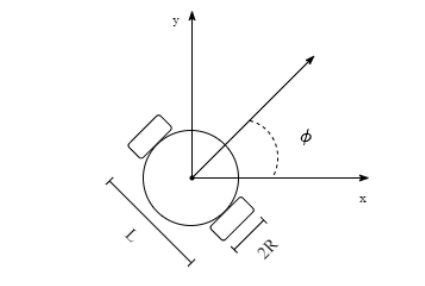
\includegraphics[scale=0.8]{chapter2/image/2banh.png}
%     \caption{Mô hình robot 2 bánh vi sai}
%     \label{fig:L298}
% \end{figure}
% Robot được coi là một chất điểm chuyển động trong đồ thị 2D dựa vào hệ quy
% chiếu tọa độ và hướng, như vậy tọa độ của robot i được xác định bởi ba thành phần
% $P(x,y,\theta)$ tốc độ $\overrightarrow{V}(x_{V},y_{V},\theta_{V})$ của robot i sẽ bằng vi phân tọa độ của P:
% \begin{equation}
%     \begin{aligned}
%     \left\{ \begin{array}{c}
%     x_{V}=\dfrac{\Delta x}{\Delta t}\\[1.5ex]
%     y_{V}=\dfrac{\Delta y}{\Delta t}\\[1.5ex]
%     \theta_{V}=\dfrac{\Delta\theta}{\Delta t}
%     \end{array}\right.
%     \end{aligned}
%     \label{eqn:xytheta}
% \end{equation}

% Với mô hình robot được thiết kế hình tròn, hai động cơ được lắp đặt ở hai bên
% giúp tâm robot nằm ở chính giữa. Với $\overrightarrow{V}(x_{V},y_{V},\theta_{V})$ là vector vận tốc mong muốn của robot, chúng ta có thể sử dụng một mô hình động học dành cho robot hai bánh vi sai.
% Vận tốc bánh trái $\omega_{L}$ là bánh phải $\omega_{R}$ được tính như sau:
% \begin{equation}
%     \begin{aligned}
%         \left\{ \begin{array}{c}
%         \omega_{L}=|\overrightarrow{V|}-\zeta*\dfrac{\theta_{t+1}-\theta_{t}}{\Delta_{t}}\\
%         \omega_{R}=|\overrightarrow{V|}+\zeta*\dfrac{\theta_{t+1}-\theta_{t}}{\Delta_{t}}
%         \end{array}\right.
%     \end{aligned}
%     \label{eqn:wlwr}
% \end{equation}

% Với hằng số $\zeta$ là hệ số điều chỉnh cố định, $\theta_{t+1}$ và $ \theta_{t}$
% là góc giữa hướng của robot
% và trục 0y tại thời điểm t + 1 và t